\chapter{A Implementação}

Conforme mencionado na seção 1.3, como aplicação prática para demonstrar os novos métodos para desenvolvimento ágil de sistemas web, foi implementado um sistema robusto para criação e manutenção de eventos batizado de EVNTs. Sempre com o objetivo de acelerar o processo de produção, foram utilizadas gemas, as quais serão explicadas com mais detalhes adiante.

\section{Funcionalidades}

A figura ~\ref{fig:esquemaapp} visa apresentar de forma geral (através de um fluxo de ações do usuário) as funcionalidades do sistema, que serão detalhadas através das subseções a seguir.

\begin{figure}[H]
\centering
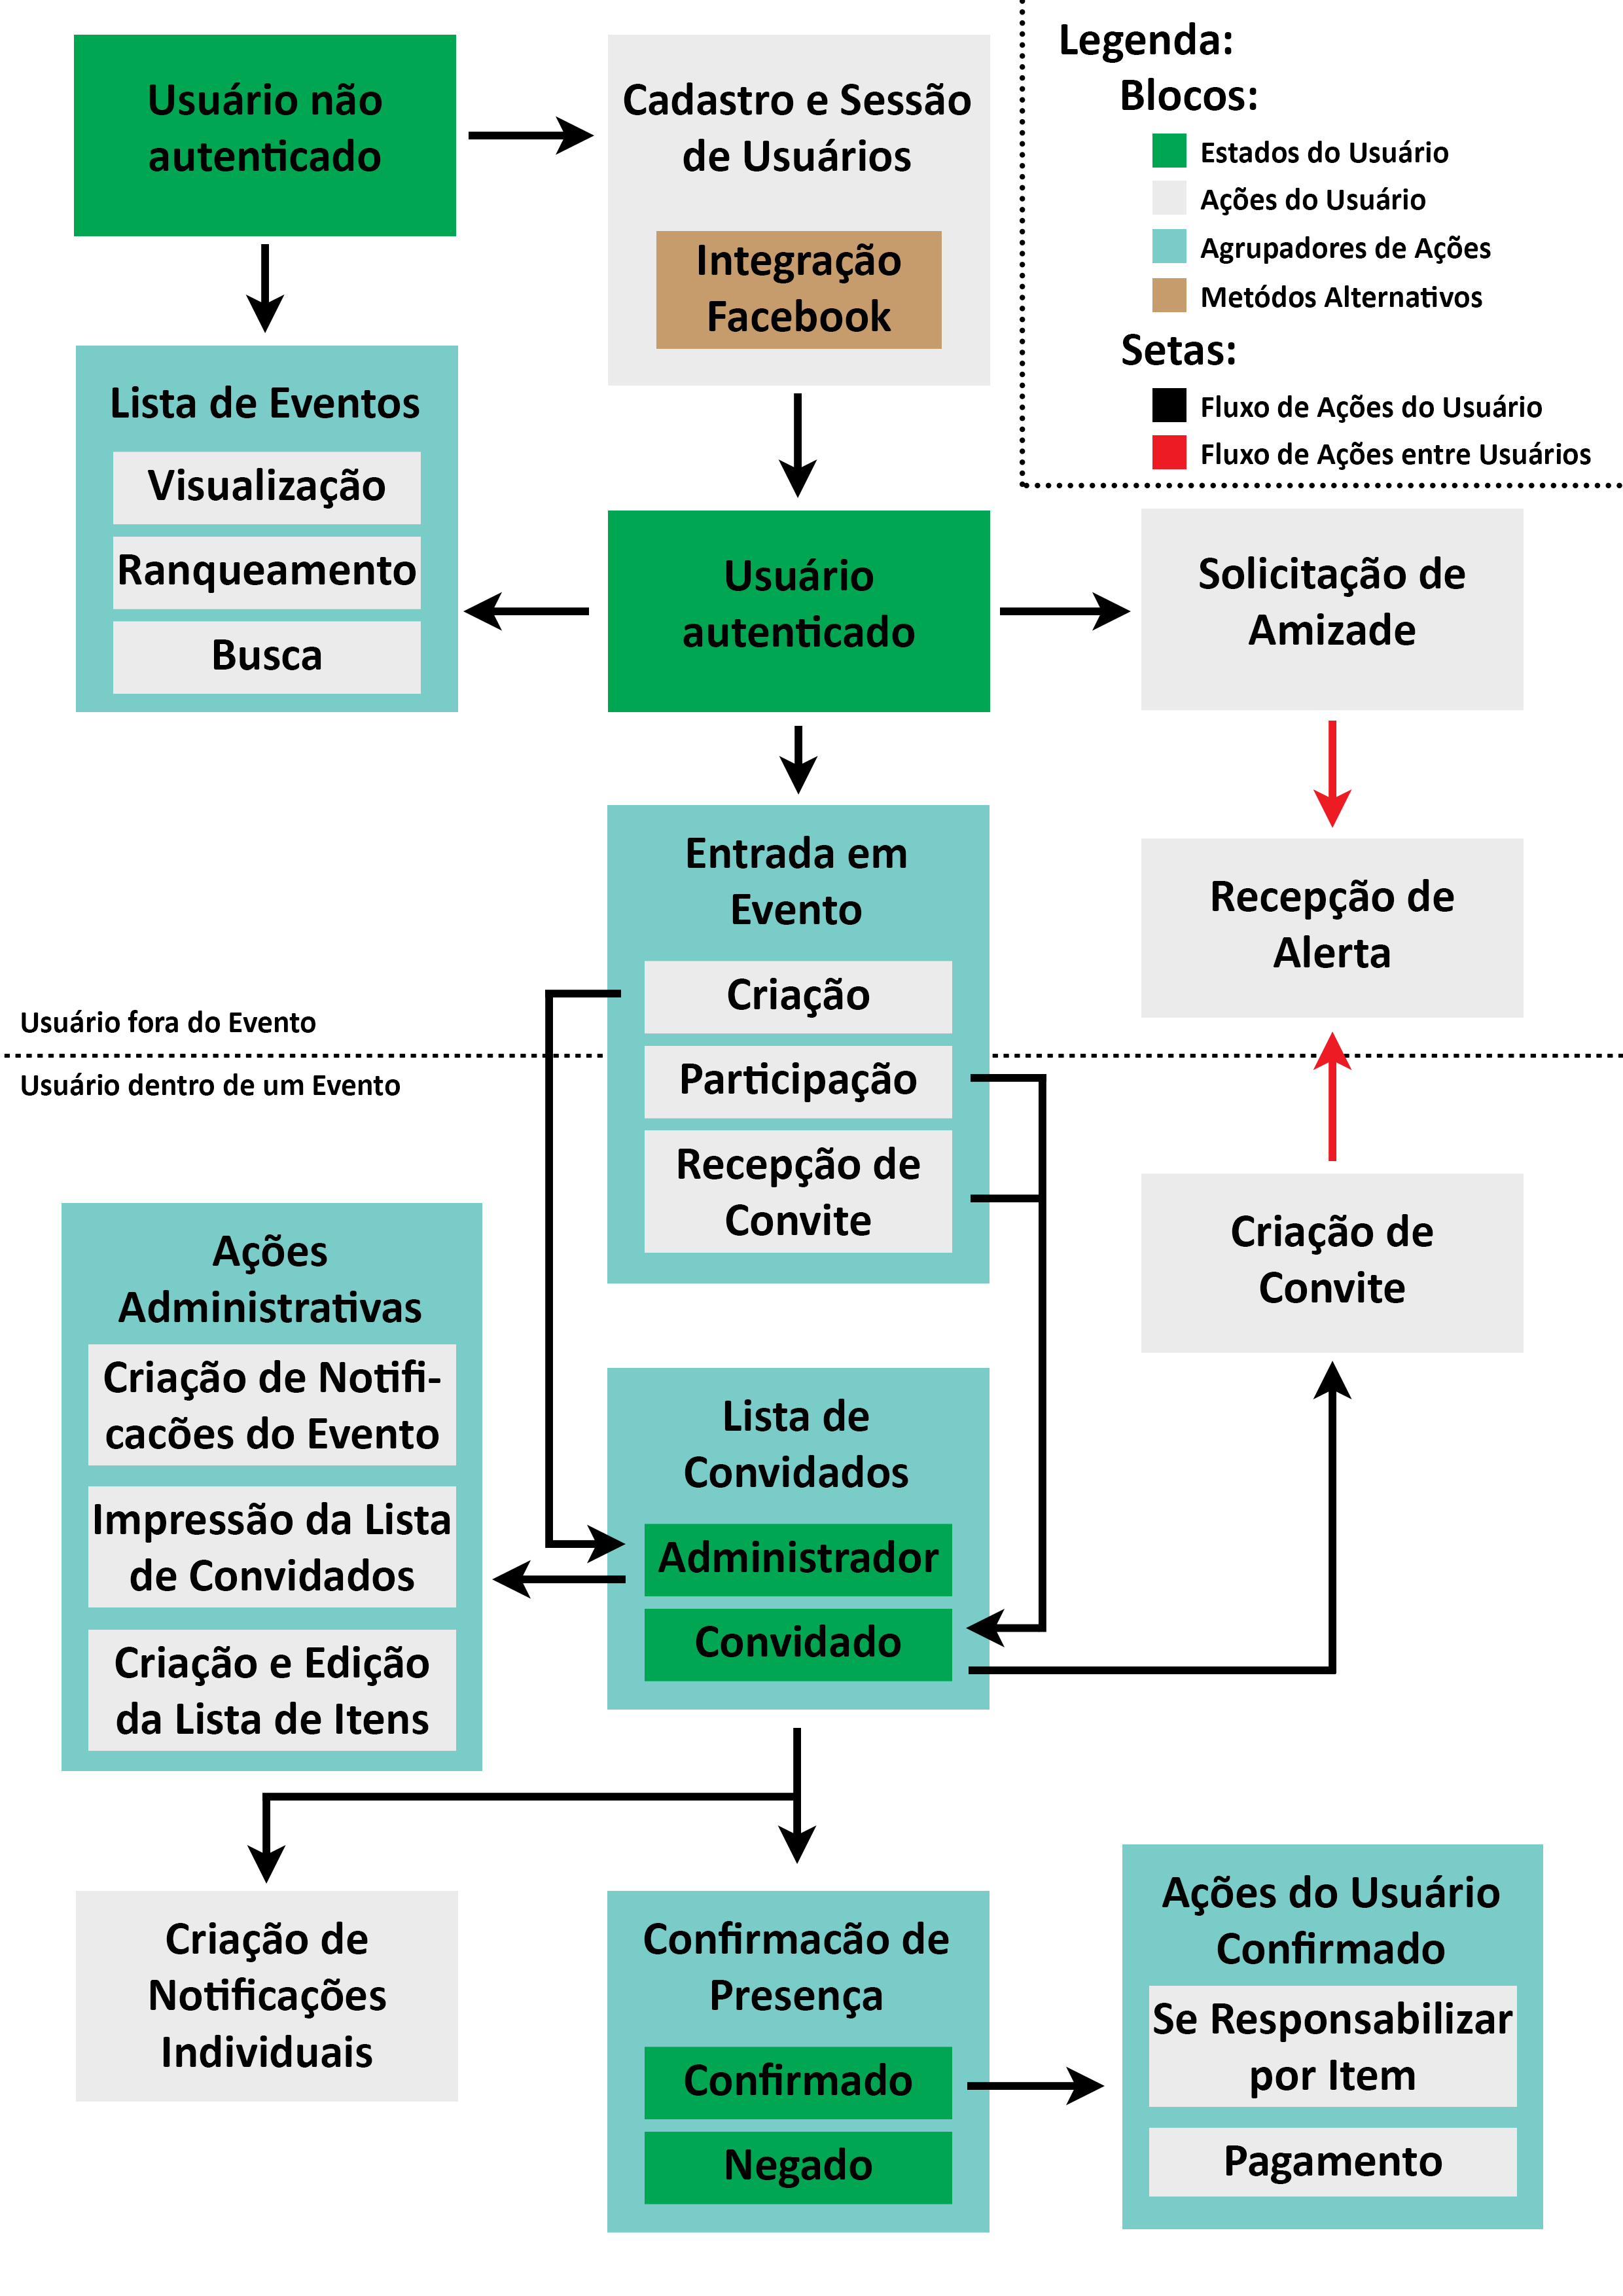
\includegraphics[width=1\textwidth]{figs/esquema_app}
\caption[\textit{Fluxo de ações do usuário no sistema}.]
{Fluxo de ações do usuário no sistema.}
\label{fig:esquemaapp}
\end{figure}

\subsection{Cadastro e Sessão de Usuários}

O projeto tem como objetivo prover funcionalidades aos usuários, tornando-os parte essencial para o bom funcionamento do sistema. Para poder identificá-los e realizar tarefas relacionadas a usuários específicos, é necessário existir sistemas de cadastro e sessão. Basicamente um sistema de cadastro consiste em um formulário que viabiliza a criação de um novo usuário no banco de dados. Um sistema de sessão, por sua vez, permite que ao retornar, esse usuário use um \textit{login} (nome ou e-mail) e uma senha, cadastrados anteriormente, para se identificar.

Por ser um módulo comum em diversos sistemas, existem muitas bibliotecas que tentam facilitar o seu desenvolvimento. No caso do Rails, a gema mais difundida, que também foi utilizada no projeto, se chama Devise~\cite{devise}.

\subsubsection{Devise}

O Devise é uma solução bastante completa para toda a parte de autenticação de usuários. Primeiramente, é muito fácil de ser configurado e é completamente personalizável, garantindo sua popularidade. Vale ressaltar que o recurso gerado pelo Devise (o usuário) é construído seguindo o padrão RESTful, tornando-o ainda mais atrativo. Dentre suas vantagens e funcionalidades estão:

\begin{itemize}
\item Segurança

Senhas criptografadas, com o custo de criptografia personalizável.

\item Histórico

Aliado também à segurança, o Devise já traz informações de data do último acesso, IP de acesso, entre outras.

\item Validação

O e-mail (campo padrão para \textit{login}) e a senha são validados automaticamente.

\item Confirmação por E-mail

Opção que faz com que o usuário receba um e-mail após o início do cadastro, onde o mesmo é finalizado, garantindo que o usuário é, de fato, dono do e-mail.

\item Manter Logado

Módulo que implementa a criação de um cookie no computador do usuário para que sua sessão seja criada automaticamente na próxima vez que retornar ao site.

\item Tempo Limite

O Devise permite o uso de um tempo máximo de inatividade para a sessão, terminando-a automaticamente ao final do prazo.

\item Trancamento de Conta

Outra funcionalidade implementada é a de trancamento de conta, para o caso de muitas tentativas sucessivas mal sucedidas de acesso em sequência. Um e-mail com instruções para destrancar é enviado automaticamente ao e-mail cadastrado, no momento do trancamento.
\end{itemize}

\subsubsection{Filepicker}

Uma parte muitas vezes complicada de sistemas é a utilização de fotos do perfil, sendo necessária a criação de uma parte de upload, hospedagem de arquivos e muitas vezes processamento da imagem como cortes e lógicas para encaixá-la ao layout. Para isso, utilizamos uma ferramenta bastante interessante chamada Filepicker.io~\cite{filepicker}. Todo o processo fica por conta da ferramenta, sendo cobrada uma taxa para tráfegos acima de 5000 fotos/mês. É bastante personalizável e permite além de upload de fotos do próprio computador, acesso a fotos de outros lugares como o Facebook, Google+, Dropbox, entre outros.

\subsection{Integração com Redes Sociais}

Para melhorar ainda mais a experiência do usuário em um sistema web, é muito comum usar contas compartilhadas, evitando que o usuário tenha que lembrar de mais um e-mail e senha. Dessa forma, foi implementada a possibilidade de cadastro e sessão utilizando a conta do Facebook do usuário. Uma gema muito útil e conhecida para isso é o Omniauth-facebook~\cite{omniauth-facebook}, atrelado ao Omniauth~\cite{omniauth}. É necessária a criação de um aplicativo no Facebook Developer (https://developers.facebook.com/) para configurar o Omniauth com uma chave de identificação e senha. Além da utilidade de cadastro e abertura de sessão, o Facebook também provê informações sobre a conta do usuário, mediante autorização, que podem ser úteis na aplicação.
Por ter se tornado popular, até mesmo o Devise implementou uma funcionalidade de integração com o Omniauth, gerando assim uma solução muito robusta e completa.

\subsection{Eventos e Lista de Convidados}

Os eventos são a parte mais importante do projeto, já que tudo gira ao redor deles. Basicamente são instâncias que devem conter informações sobre local, data, hora, preço e privacidade. Além disso, usuários devem ser capazes de criar eventos, confirmar ou negar presença nos mesmos e convidar outros usuários a participarem deles. É importante também a ferramenta de impressão da lista de confirmados para o organizador, de forma a facilitar sua vida no dia do evento.

\subsubsection{Privacidade}
Foram implementados três tipos de privacidade para os eventos:

\begin{itemize}
\item Públicos

Eventos vistos e encontrados por qualquer usuário. Qualquer um pode confirmar presença e convidar pessoas.

\item Privados

Eventos onde somente pessoas convidadas pelo organizador podem ver e confirmar presença, porém, convidados não podem convidar.

\item Convidativos

Parecido com o privado, porém, neste caso os convidados podem convidar mais usuários.
\end{itemize}

\subsubsection{Preço}
O preço do evento depende basicamente de três informações.

\begin{itemize}
\item Preço Fixo

Valor constante, que deve ser pago por todos os confirmados.

\item Preço Compartilhado

Valor constante a ser dividido entre todos os confirmados.

\item Preço de Itens

Valor que representa o somatório dos preços dos itens. Este caso será explicado com mais detalhes na próxima seção.
\end{itemize}

\subsection{Lista de Itens}

Essa funcionalidade é um dos principais diferencias do sistema desenvolvido com relação ao que existe no mercado. Em suma, trata-se de uma lista de itens (como refrigerantes, bola de futebol ou aparelho de som)  que são necessários para a realização do evento. Uma vez criada, usuários podem se tornar responsáveis por itens, isto é, se comprometem a levar o item no dia do evento. Os itens podem ter quantidades específicas, possibilitando que a responsabilidade sobre um mesmo item seja dividida entre mais de um usuário.

Além disso, itens podem possuir preço. Neste caso, o valor somado da lista também será dividido entre os confirmados no evento. O valor de um item, atrelado à quantidade adquirida por um responsável, será descontado do valor a ser pago por este usuário.

\subsection{Pagamento}

Outro diferencial do sistema é a possibilidade de pagamento através do mesmo, dando uma garantia muito maior ao organizador da presença de seus convidados e suporte ao planejamento financeiro do evento. Para que não ocorram problemas, é importante notar que eventos com custo compartilhado ou lista de itens pagos, não poderá ter pagamentos através do sistema, uma vez que, nestes casos, o valor se altera à medida que novos usuários confirmam presença.

O pagamento ocorrerá através do Paypal~\cite{paypal}, uma ferramenta simples e segura de realizar pagamentos na Internet. Eles possuem uma API fácil de utilizar e bastante completa, incluindo até mesmo um ambiente para testes. Sua única desvantagem é que o usuário será redirecionado para um site externo ao sistema na hora de pagar, piorando a experiência do usuário.

O dinheiro irá para a conta do EVNTs, e, após a realização do evento, será transferido para a conta bancária cadastrada pelo usuário. Essa transferência, em um primeiro momento, ocorrerá de forma manual, porém em trabalhos futuros será implementado um sistema automático para isso. Além disso, diversos casos de segurança (principalmente fraudes) ainda não estão sendo contemplados e serão resolvidos também no futuro.

\subsection{Amizades}

Para facilitar a parte de convites para o evento, foi implementado um módulo de amizades, que permite um relacionamento entre dois usuários. Basicamente, um usuário envia uma solicitação de amizade a outro usuário que pode aceitá-la, recusá-la ou até mesmo recusá-la para sempre. Uma vez que a solicitação foi aceita, a amizade é criada. Desta forma, torna-se possível convidar o amigo para eventos de forma simples e direta.

Como já existe a integração com o Facebook no momento do cadastro, a lista de amigos da rede social será aproveitada de forma a automaticamente recriar as amizades dentro do sistema EVNTs, reduzindo o trabalho do usuário.

\subsection{Notificações e Alertas}

Para que o evento não entre no esquecimento, foi implementado um módulo de notificações. A ideia é que o organizador possa criar notificações a serem enviadas para todos os confirmados no seu evento e que cada usuário possa criar notificações individuais para si. Porém, o usuário pode se subscrever ou não às notificações gerais, de forma a evitar casos não desejáveis.

A notificação será na forma de um e-mail que será enviado na data desejada para o usuário indicando a data, horário, local do evento e os itens que aquele usuário deverá levar. Para que ela seja programada para uma data posterior, utilizamos uma gema chamada Delayed Jobs~\cite{delayed_jobs}, que permite de forma bastante simples, executar ações assíncronas no sistema, seja por um sistema de fila, isto é, várias ações para serem executadas em sequência, ou por um sistema de data marcada. Seu funcionamento se dá através de uma tabela no BD onde as ações ficam guardadas e um sistema que verifica a existência de tarefas a serem executadas nessa tabela.

Além disso, há um sistema de alertas para convites de eventos e solicitações de amizades pendentes. Os alertas serão visíveis apenas na aplicação.

\subsection{Ranqueamento de Eventos}

Com o objetivo de divulgar eventos públicos, foi gerado uma lógica para ranqueamento de eventos, com o intuito de, na página inicial do sistema, exibir listas de eventos organizadas de forma interessante ao usuário. Foram implementados dois tipos de listas:

\begin{itemize}
\item Selecionada por distância em relação ao usuário e número de confirmados no evento.

Neste caso, o cálculo da distância é feito através do uso da gema Geocoder~\cite{geocoder}, que permite desde a captura da localização até mesmo o cálculo da distância para um certo ponto geográfico. Utilizamos também a API do Google Maps~\cite{google_maps} que permite visualizações de mapas e um ``auto completar'', utilizado no cadastro de eventos que permite adquirir uma latitude e longitude baseados no endereço.

\item Selecionada pela quantidade de amigos confirmados no evento.
\end{itemize}

Nos dois casos, as listas estarão ordenadas pela data de realização do evento, eliminando eventos ocorridos, proporcionando uma visualização clara e objetiva dos eventos que estão por vir.

\section{Modelos}

Nesta seção, será mostrado em maior detalhe os principais modelos do projeto. Os modelos foram a primeira parte a ser construída do sistema, juntamente com seus testes, já que foi utilizada a metodologia TDD.

Para ajudar no entendimento desta seção, a figura ~\ref{fig:Modelo de Dados - Tabelas e Relacionamentos} pode ser utilizada.

\begin{figure}[H]
\centering
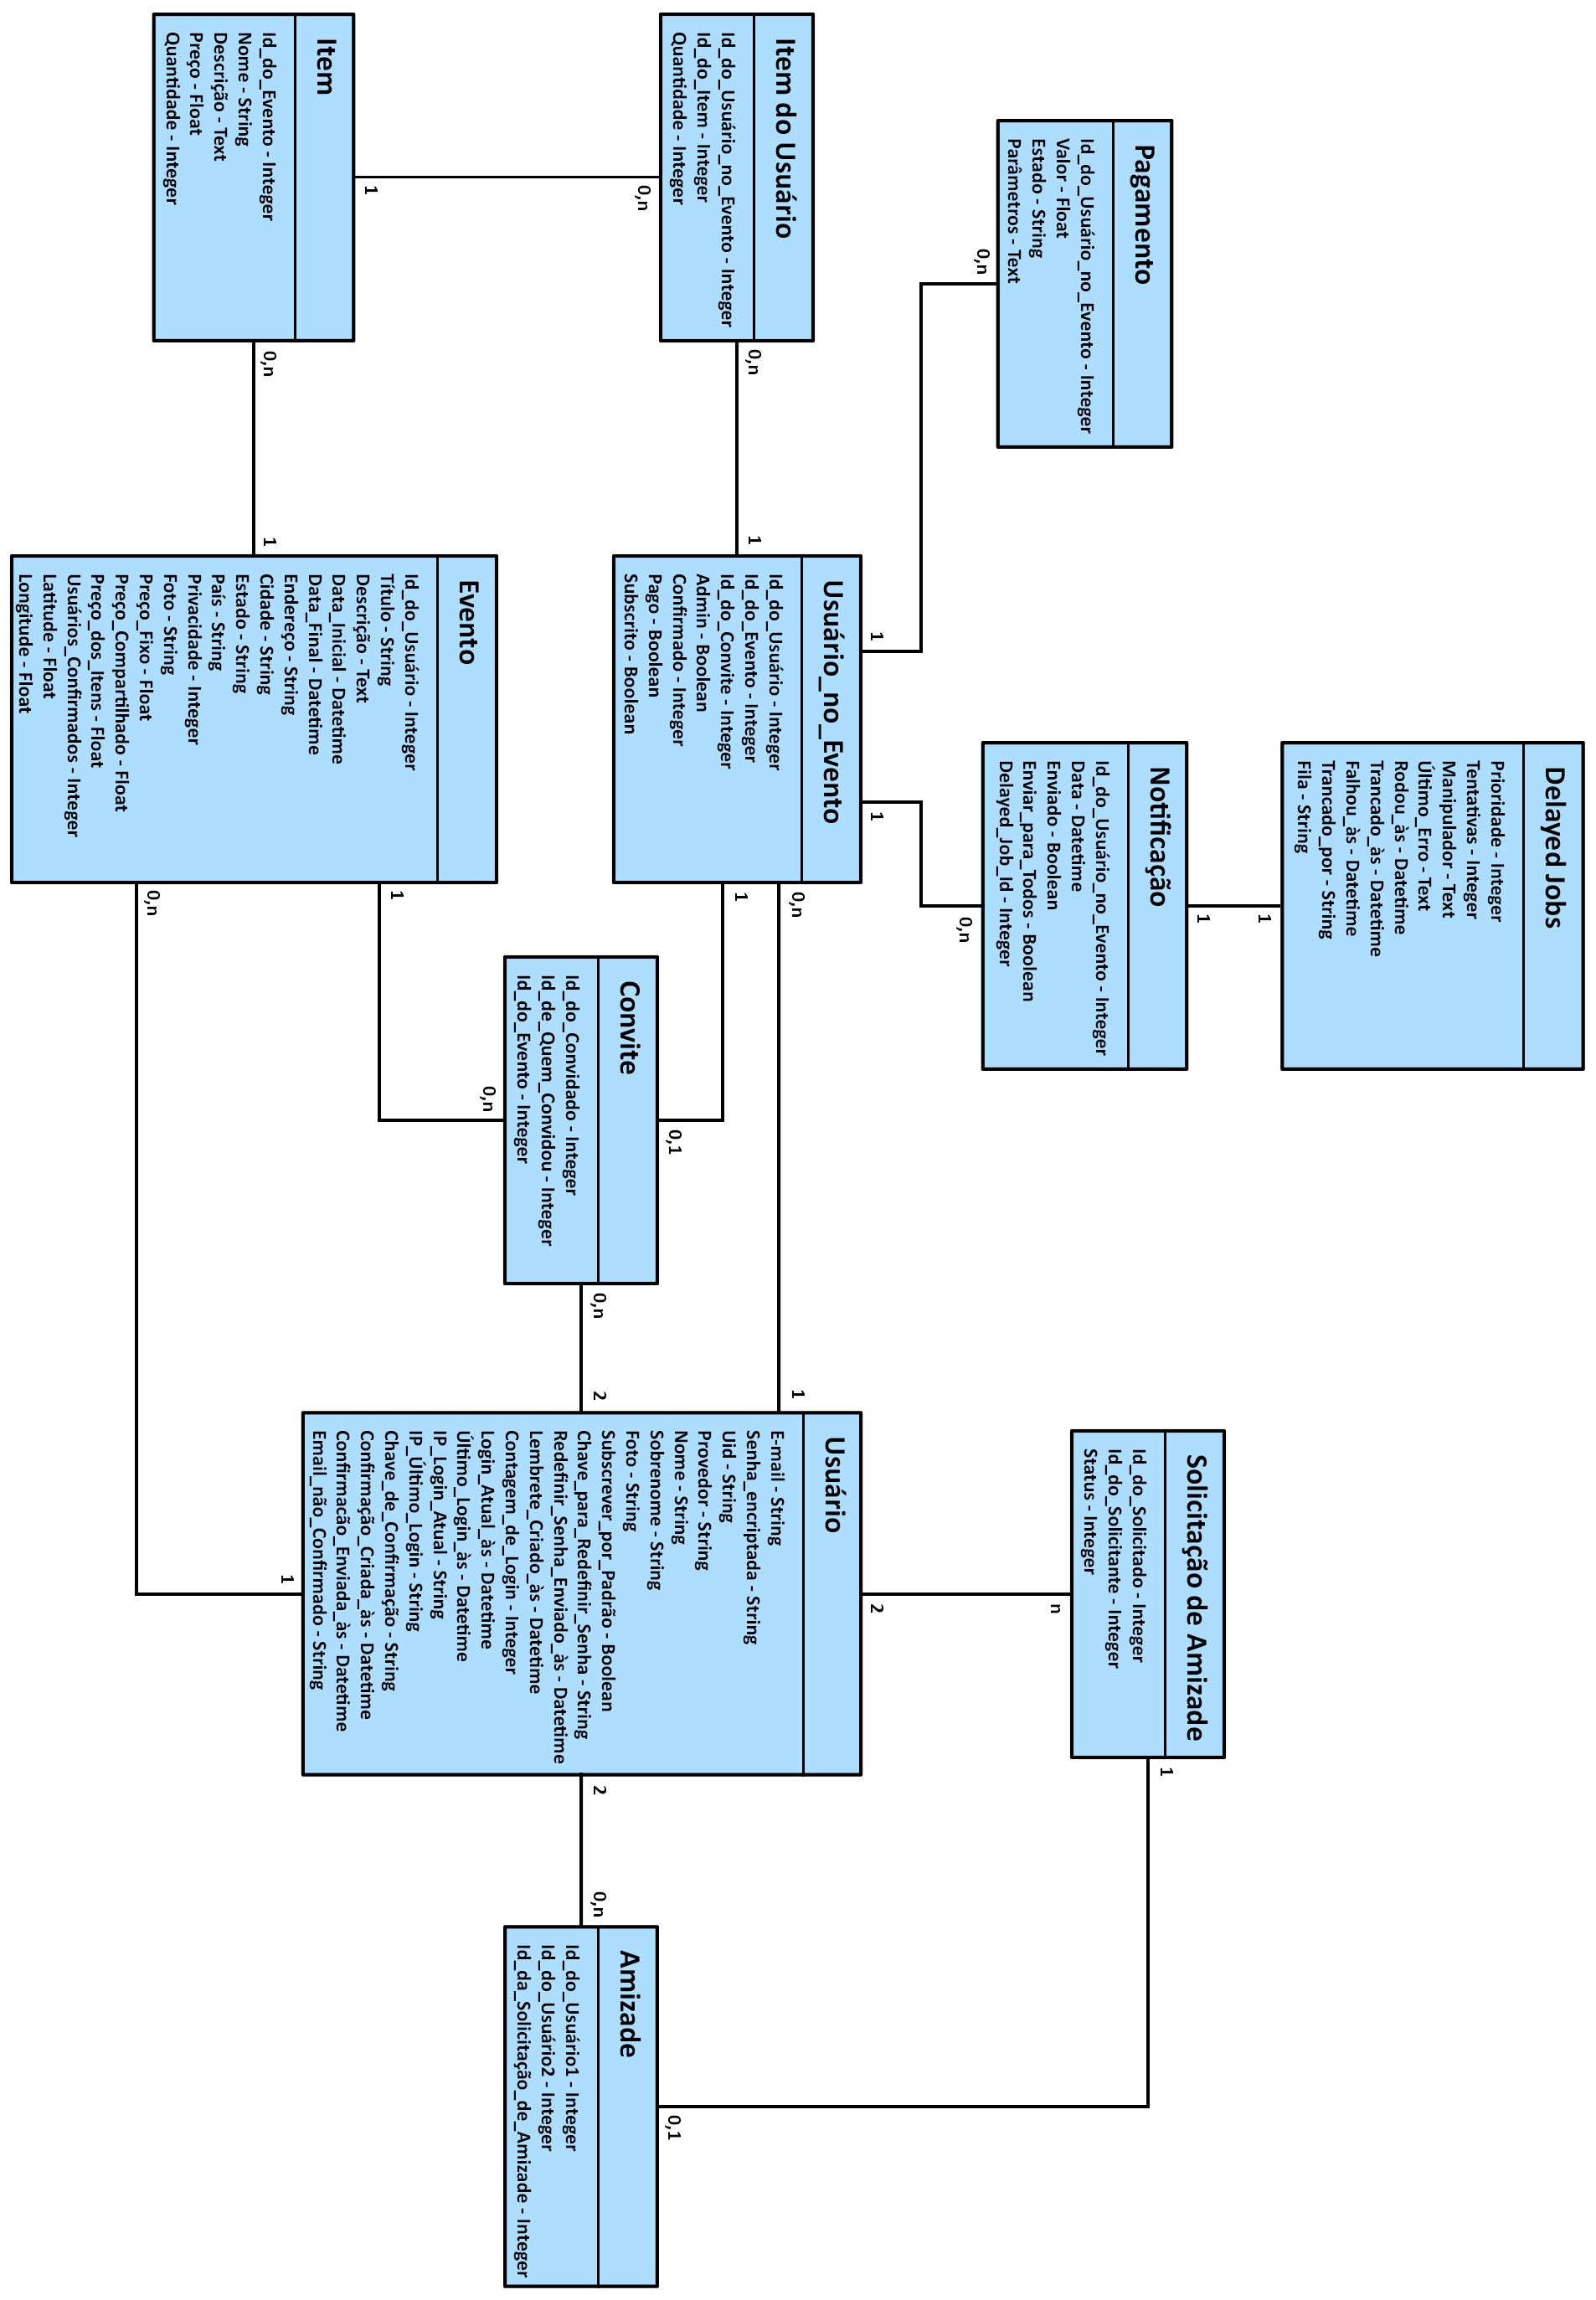
\includegraphics[width=1\textwidth]{figs/modelo_de_dados}
\caption[\textit{Modelo de Dados - Tabelas e Relacionamentos}.]
{Modelo de Dados - Tabelas e Relacionamentos.}
\label{fig:Modelo de Dados - Tabelas e Relacionamentos}
\end{figure}

\subsection{Usuário}

A tabela de usuário possui diversos campos que foram criados devido às funcionalidades do Devise. Primeiramente, o e-mail e senha, já que são os campos padrão do Devise para identificação do usuário. Além disso, por ter sido utilizada a funcionalidade de confirmação por e-mail, os campos \textit{chave\_de\_confirmação}, \textit{confirmação\_criada\_às}, \textit{confirmação\_enviada\_às} e \textit{email\_não\_confirmado} foram criados pela gema. Os campos \textit{contagem\_de\_login}, \textit{login\_atual\_às}, \textit{último\_login\_às}, \textit{ip\_login\_atual} e \textit{ip\_último\_login} são utilizados pela biblioteca para manter o histórico e segurança. Por último, os campos \textit{chave\_para\_redefinir\_senha} e \textit{redefinir\_senha\_enviado\_às} são utilizadas para, com segurança, ter a funcionalidade de ``esqueci minha senha''.

Para o bom funcionamento da integração com o \textit{login} do Facebook, são criados os campos \textit{uid} e o \textit{provedor}. O \textit{provedor} simplesmente guarda por qual provedor estamos fazendo o acesso, para o caso de existir o \textit{login} por outros meios além do Facebook. Já o campo \textit{uid} guarda a identificação do usuário dentro da rede a qual ele pertence.

Os outros campos são bastante intuitivos. O único que vale a atenção é o \textit{subscrever\_por\_padrão}, que tem como objetivo definir se, por padrão, ao entrar num evento o usuário estará subscrito ou não às notificações gerais do mesmo.

\subsection{Evento}

A tabela de eventos é um ponto central do sistema. Como buscas de eventos são bastante comuns, algumas variáveis foram adicionadas à tabela para agilizar esse processo. Entre elas, \textit{cidade}, \textit{estado} e \textit{país} que têm por objetivo restringir os eventos por localidade, \textit{preço\_dos\_itens} e o número de confirmados para evitar o acesso a outras tabelas em funções muito requisitadas e a \textit{latitude} e \textit{longitude}, para rapidamente poder calcular a distância do usuário até o local do evento.

A validação dos campos de eventos é um ponto importante a ser discutido. Como existem tipos de privacidade e de pagamento, é importante que sempre exista a garantia de que esses dados estão consistentes entre si. Além disso, por possuir informações de valores relacionados a outras tabelas, é sempre importante garantir que ao editar um evento, esses valores estejam sempre corretos.

\subsection{Usuário no Evento}

Essa tabela é a terceira tabela essencial para o funcionamento do sistema, já que é ela que relaciona as duas entidades mais importantes (o evento e o usuário). Todas as tabelas que são relacionadas a um usuário no caso dele estar em um evento, se relacionam diretamente com esta tabela, facilitando a implementação de funções relacionadas a esta situação, como um pagamento ou uma notificação.

Além dos campos que identificam seus relacionamentos, essa tabela possui alguns campos importantes:

\begin{itemize}
\item \textit{Admin}

Define se esse usuário tem direitos administrativos sobre o evento, como no caso de ser o organizador.

\item \textit{Confirmado}

Deve ter um valor que indique se o usuário vai, não vai, ou ainda não respondeu se vai ao evento.

\item \textit{Pago}

Evita o acesso a todos os pagamentos (ou tentativas mal sucedidas de pagamento) na hora de saber se usuário já pagou. É importante notar que essa variável possui uma validação importante, já que, além de depender da tabela de pagamentos, é uma parte sensível do fluxo do sistema.

\item \textit{Subscrito}

Define se o usuário receberá as notificações gerais do evento ou não. Vale ressaltar que, por padrão, essa variável assume um valor relativo à variável \textit{subscrever\_por\_padrão} do usuário em questão.
\end{itemize}

\subsection{Notificação}

A tabela de notificação possui algumas singularidades. Primeiramente, o campo \textit{Enviar\_para\_Todos} que é o que diferencia uma notificação geral de um evento para uma notificação personalizada do usuário. É importante notar, que mesmo a notificação geral pertence a um \textit{Usuário\_no\_Evento}, porém, no caso de ser geral, pertencerá ao \textit{Usuário\_no\_Evento} referente ao organizador do evento.

Além disso, para se integrar com a gema Delayed Jobs citada anteriormente, é necessário que exista um campo que relacione a tabela de notificação com um registro na tabela de \textit{Delayed Jobs}. No momento que este registro na tabela de \textit{Delayed Jobs} disparar, ele vai verificar a notificação correspondente e de fato notificar os usuários. Caso o \textit{Enviar\_para\_Todos} seja verdadeiro, essa tarefa irá enviar um e-mail para todos os participantes do evento.

\subsection{Outras Tabelas}

Por serem tabelas mais simples e óbvias, não serão explicitados detalhes. Vale notar que as tabelas \textit{Convite}, \textit{Solicitação\_de\_Amizade} e \textit{Amizade} relacionam dois usuários diferentes entre si. Cada uma com objetivos diferentes.

\subsection{Extras}

Um ponto importante a ser levantado é o relacionamento entre as tabelas. Alguns registros devem ser automaticamente criados a medida que determinadas ações são disparadas. Por exemplo, uma amizade deve ser criada automaticamente quando uma solicitação de amizade é registrada como aceita. Dessa forma, a lógica geral de integração entre os modelos já estará praticamente pronta, deixando para os controladores apenas as ações que de fato ocorrem com a interação de um usuário com o sistema.

\section{Controladores}

Uma vez tendo os modelos prontos e sendo validados, o projeto já está bem encaminhado e então torna-se necessária a criação dos controladores, que recebem as requisições feitas pelos usuários e definem o que deve ser feito. Como citado anteriormente, durante a implementação do projeto usou-se a metodologia RESTful, tornando os controladores bem simples e bem intuitivos, já que quase sempre possuem apenas ações de \textit{Index}, \textit{Show}, \textit{New}, \textit{Create}, \textit{Edit}, \textit{Update} e \textit{Destroy}. Apenas em dois casos essa lógica não se mantém:

\begin{itemize}
\item Busca de evento

Foi criado uma ação especial \textit{Search} para a busca de eventos, deixando o código mais limpo e organizado.

\item Alteração de subscrição

Por ser uma tarefa bem simples e não necessitar de validação por conta do modelo, foi definida uma ação para alterar a subscrição de um usuário às notificações do evento ao invés de usar o método padrão \textit{Update}.
\end{itemize}

Um ponto a ser lembrado é que, por padrão, controladores respondem com HTML, porém em casos de requisições AJAX, essa resposta deve ser dada de forma diferente, seja por um objeto JSON, um XML ou até mesmo Javascript diretamente. Inclusive, é possível configurar um controlador para responder a chamadas diferentes com formatos distintos, ou seja, responder tanto para requisições AJAX quanto a requisições HTTP padrões.

\section{Visões}

Para agilizar o desenvolvimento do \textit{frontend} do sistema, foi utilizado o Bootstrap~\cite{bootstrap}, um \textit{framework} de CSS e Javascript muito intuitivo, de fácil utilização e poderoso. Basicamente, o Bootstrap é um conjunto de classes de estilo (CSS) e funções Javascript a serem utilizadas. Um exemplo de um resultado alcançado rapidamente utilizando bootstrap pode ser observado na figura ~\ref{fig:pagvisuevento}. Trata-se da página de visualização de um evento dentro do sistema implementado. As barras de navegação (no topo e final da página), estilo dos botões, posicionamento em colunas e linhas, campos de preenchimento, entre outros elementos, estão seguindo o padrão do Bootstrap, sendo perceptível o poder da ferramenta e o motivo do seu uso.

\begin{figure}[H]
\centering
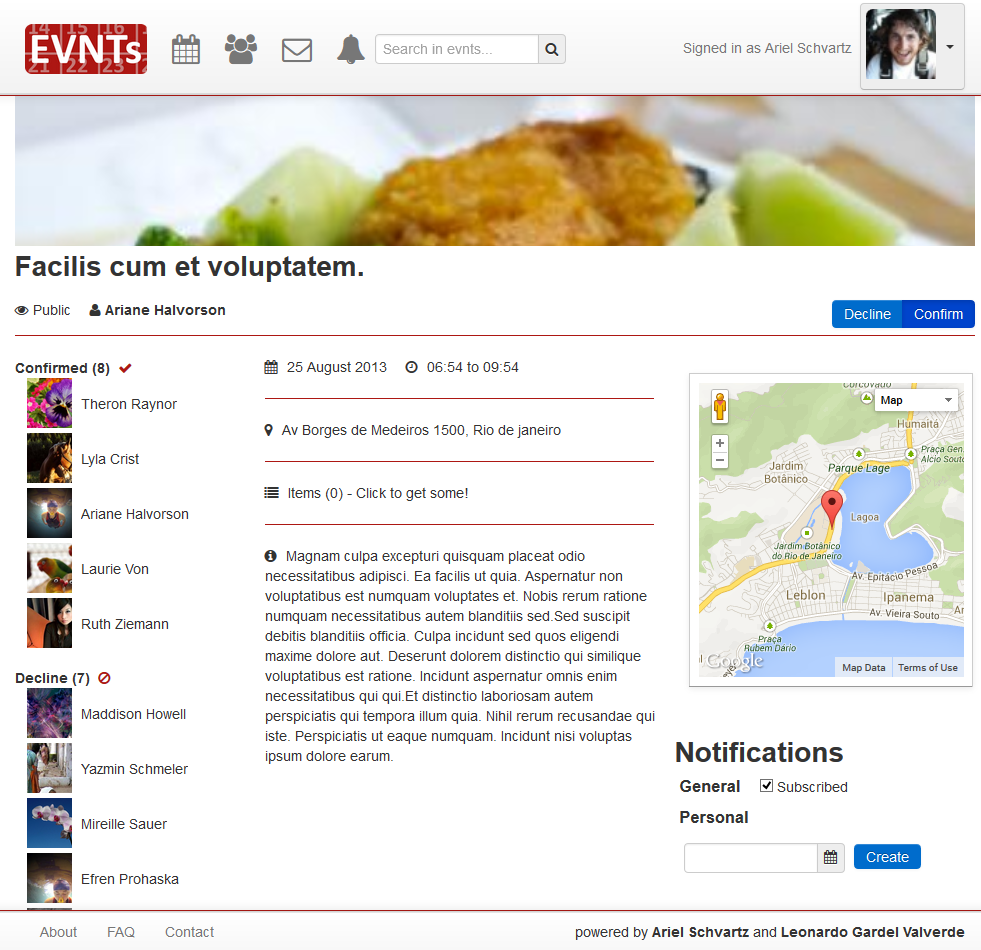
\includegraphics[width=1\textwidth]{figs/event_show}
\caption[\textit{Página de Visualização de Evento}.]
{Página de Visualização de Evento.}
\label{fig:pagvisuevento}
\end{figure}

Além disso, para gerar essa visualização interativa do mapa de localização, foi utilizada a API do Google Maps. Sua utilização é gratuita enquanto o tráfego for pequeno e sua implementação, que se dá através de uma biblioteca em Javascript, é muito fácil e bem documentada.

Outra ferramenta importante para o layout do projeto, foi o Font Awesome~\cite{font_awesome}, que basicamente é biblioteca em CSS que fornece uma fonte que ao invés de conter letras, contém ícones. Dessa forma, os ícones têm qualidade de vetor e são muito leves, já que não são imagens. Seu uso é totalmente gratuito, tornando-o ainda mais atrativo. Ao olhar a figura ~\ref{fig:pagvisuevento}, da página do evento, percebe-se que o uso de ícones torna o site ainda mais agradável e bonito.

Outra questão importante sobre as visões foi o alto uso de AJAX e Javascript. O seu uso evita o carregamento repetidas vezes de páginas completas, reduzindo a quantidade de conteúdo carregado sem necessidade. Dessa forma, obtém-se uma melhora na experiência do usuário, que tem uma resposta mais rápida de suas ações. Outro aspecto bom do uso de Javascript e JQuery é a utilização de animações, criando um sistema mais fluido e agradável. Porém, em contrapartida, usuários podem desativar o Javascript de seus navegadores (principalmente em celulares), apesar de não ser muito comum.

\section{Teste}

Foram implementados testes unitários e funcionais, que representam os testes dos modelos e controladores, como explicado anteriormente.

\subsection{Teste dos Modelos}

Os testes de modelo tem como foco:
\begin{itemize}
\item Validações

Verificar se casos não consistentes de modelos realmente estão sendo validados e negados, enquanto casos consistentes são aceitos pelo sistema. Esses testes garantem registros sempre consistentes no BD.

\item Chamadas de retorno

Diversos modelos devem realizar ações antes ou após serem salvos. Por exemplo, um item, ao ser salvo, deve alterar a variável \textit{Preço\_dos\_Itens} do evento a qual esse item pertence. Neste caso, o valor final da variável deve ser testado para garantir que todas as chamadas estão acontecendo corretamente.

\item Valores padrões

Algumas variáveis devem assumir valores padrões quando o registro é inicializado. Por exemplo, um convite deve gerar um \textit{Usuário\_no\_Evento} com a variável confirmado em um valor padrão para o caso do usuário ainda não ter dado a resposta.
\end{itemize}

Para realizar os testes de modelo e simular dados consistentes e inconsistentes, foram usadas algumas gemas:

\subsubsection{Factory Girl~\cite{factory_girl}}

Permite de forma clara e organizada a criação de registros no banco de dados. Permite a criação de instâncias salvas, não salvas e até mesmo a criação de registros em cadeia, no caso da existência de relacionamentos. A ideia é basicamente criar ``fábricas'' de registros em um arquivo e nos testes apenas chama-las, criando assim um código limpo e DRY (ver seção 2.4)

\subsubsection{FFaker~\cite{ffaker}}

O FFaker, é uma segunda versão da gema Faker, porém reescrita para rodar de forma mais rápida. A ideia da gema é gerar informação básica aleatória, como por exemplo nomes, e-mails, endereços, textos, entre outros. Desta forma, é possível simular informações pseudoaleatórias para testar o sistema.

\subsubsection{Timecop~\cite{timecop}}

Essa gema basicamente permite ``viajar no tempo'' e ``parar no tempo''. Na verdade, o que acontece é que a gema simula horários possibilitando os testes que são dependentes do tempo, como no caso dos testes das notificações. Dessa forma, é possível ``viajar'' até a data onde a notificação deveria ser enviada e verificar se tudo correu bem.

\subsection{Teste dos Controladores}

Os testes dos controladores têm como foco:

\begin{itemize}
\item Rotas e Redirecionamentos

Testes que verificam se as rotas existem e estão retornando sucesso. Além disso, devem verificar que em certos casos, o usuário será redirecionado. Por exemplo, ao criar um evento, o usuário deve ser redirecionado para a página de visualização do evento que acabou de ser criado.

\item Respostas

Testes que avaliam a resposta dada pela rota, isto é, se a requisição foi por AJAX, a resposta não deve ser HTML. Além disso, é importante verificar as informações que são respondidas. Por exemplo, ao criar um novo item por AJAX, deseja-se como retorno o novo item criado, para adicioná-lo à página sem recarregá-la.

\item Permissões

Testes que avaliam casos de permissões de acesso a páginas específicas. Por exemplo, um usuário que não iniciou sua sessão ou que não faz parte de um evento privado não deveria ser capaz de acessar esse evento.

\end{itemize}

Para ajudar nestes testes, além das gemas já mencionadas, foi utilizada a gema Mocha~\cite{mocha}.

\subsubsection{Mocha}

Esta gema permite ``enganar'' o BD, simulando que qualquer instância a ser salva vai ser válida ou não. Isso ajuda muito na hora de testar rotas como o \textit{create} e \textit{update}, simulando casos de sucesso e de falha de forma fácil e rápida.

\section{Ambientes}

Existem três ambientes básicos a serem utilizados pelo sistema. O de desenvolvimento, de testes e de produção. Como o de testes é análogo ao ambiente de desenvolvimento, este não será explicado em detalhes.

\subsection{Desenvolvimento}

Para o ambiente de desenvolvimento, o SGBD utilizado é o SQLite, principalmente por ser muito leve e não precisar de nenhum tipo de configuração para funcionar. Este SGBD se torna suficiente em desenvolvimento, já que a quantidade de dados é baixa e não é necessária uma grande eficiência a nível de BD. Para utilizar o SGBD é necessário instalar a gema referente ao banco.

Neste ambiente, é muito comum o uso do IRB (\textit{Interactive Ruby Shell})
\abbrev{IRB}{\textit{Interactive Ruby Shell}}
, um prompt de comando do seu sistema, onde você pode acessar o BD, chamar funções, entre outros. Seu uso se dá principalmente pela necessidade de depurar o código.

As gemas utilizadas para o ambiente de desenvolvimento foram:

\subsubsection{Pry~\cite{pry}}

O Pry é um substituto do prompt de comando padrão do Rails, o IRB. Suas principais vantagens são a coloração de sintaxe Ruby, a velocidade (rápido comparado ao IRB) e a possibilidade de invoca-lo em tempo de execução. Esta última funcionalidade se torna extremamente necessária e importante para depurar código, já que a qualquer momento do fluxo de execução é possível travar o sistema e ter comandos Ruby a sua disposição.

\subsubsection{Letter Opener~\cite{letter_opener}}

Essa gema permite visualizar diretamente no browser, um e-mail que seria enviado. Isso evita a necessidade de configurar uma conta de e-mail no ambiente de desenvolvimento. Além de agilizar o processo de configuração do sistema e de visualização dos e-mails, a gema ainda evita que diversos e-mails sejam mandados para sua caixa de entrada.

\subsubsection{Better Errors}

Essa gema faz um trabalho bastante simples mas que ajuda muito na depuração de erros. Basicamente, a ideia é melhorar as páginas de erros. Ao invés de simplesmente uma mensagem jogada na tela, outras informações como inspeção de variáveis também são mostradas e a visualização do erro é muito mais agradável e de fácil leitura.

\subsection{Produção}

Para produção, utilizamos o Heroku~\cite{heroku}, uma plataforma de aplicativos na nuvem que permite aos desenvolvedores se focarem somente no desenvolvimento de código, sem ter de se preocupar com gerenciamento de servidores, implantação ou escala. Além disso, existe um plano gratuito, obviamente limitado, porém completo e bastante útil para testar com usuários reais em um primeiro momento. Para garantir a facilidade no momento de implantação, esta se dá através do próprio GIT se tornando rápida e fácil.

Por padrão, o Heroku usa como SGBD o Postgres, que é um banco de dados robusto e eficiente quando comparado a outros SGBDs. Portanto, foi instalada a gema do Postgres para se adequar aos requisitos do sistema.
